\documentclass{article}
\usepackage[utf8]{inputenc}
\usepackage[top=2cm, bottom=4.5cm, left=2.5cm, right=2.5cm]{geometry}
\usepackage{graphicx}
\usepackage{booktabs}
\title{ANLY601 Assignment1}
\author{Shaoyu Feng (sf865) \\
Collobrator: Mengtong Zhang (mz500) \\
Collobrator: Yunjia Zeng (yz682)
}

\date{April 2020}

\begin{document}

\maketitle

\section{Question1 Boosting} 
\begin{enumerate}
\item \textbf{Part1} \\
\begin{enumerate}
\item Q0\\
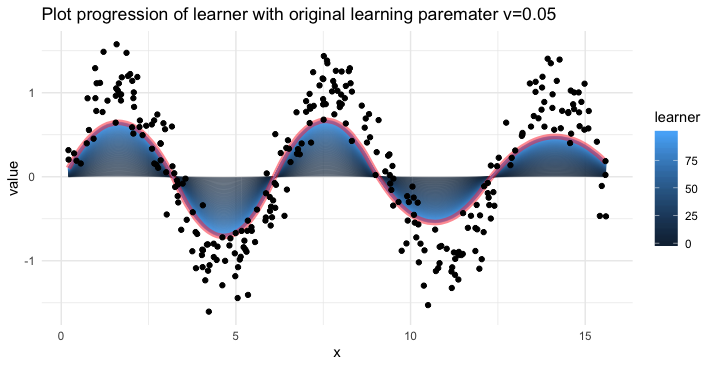
\includegraphics[width=16cm, height=10cm]{spline_learner_V_0.05.png}\\
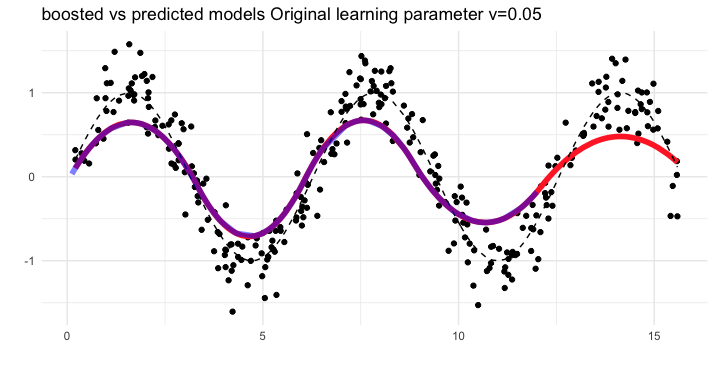
\includegraphics[width=16cm, height=10cm]{spline_prediction_v_0.05.png}\\
\item Q1 \\
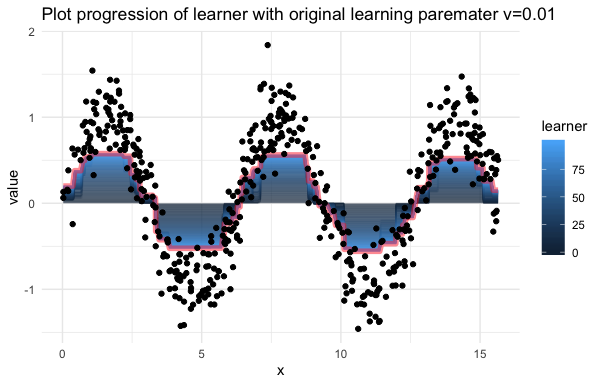
\includegraphics[width=16cm, height=10cm]{learner_v=0.01.png}\\
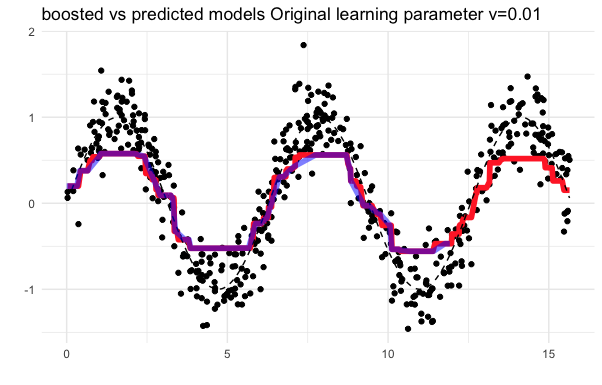
\includegraphics[width=16cm, height=10cm]{prediction_v_0.01.png}\\
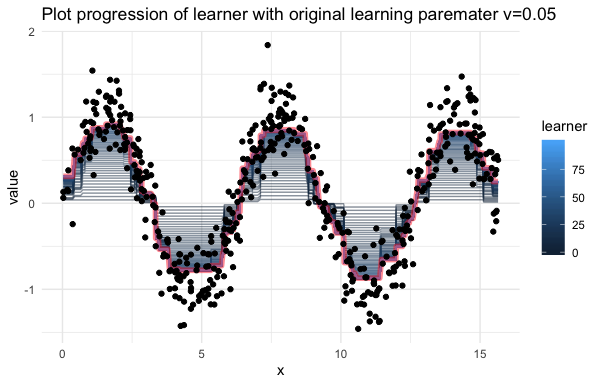
\includegraphics[width=16cm, height=10cm]{learner_v_0.05.png}\\
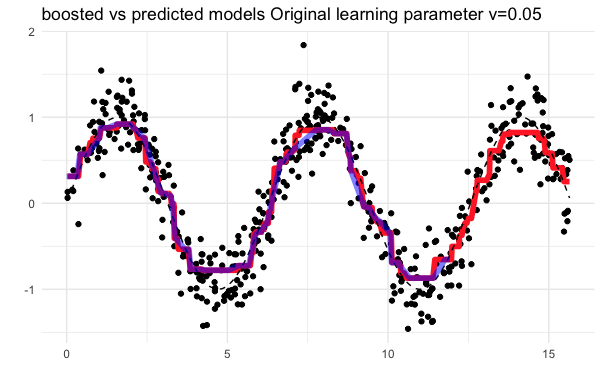
\includegraphics[width=16cm, height=10cm]{prediction_v_0.05.png}\\
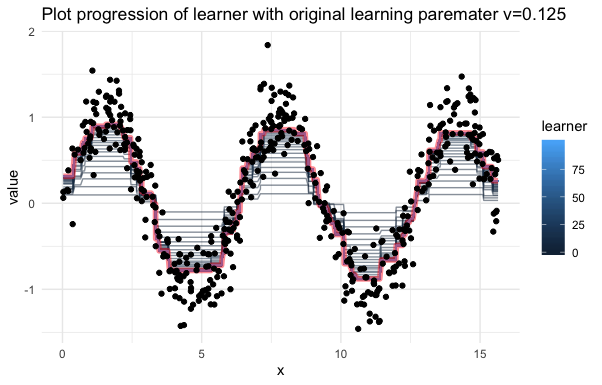
\includegraphics[width=16cm, height=10cm]{leaner_v_0.125.png}\\
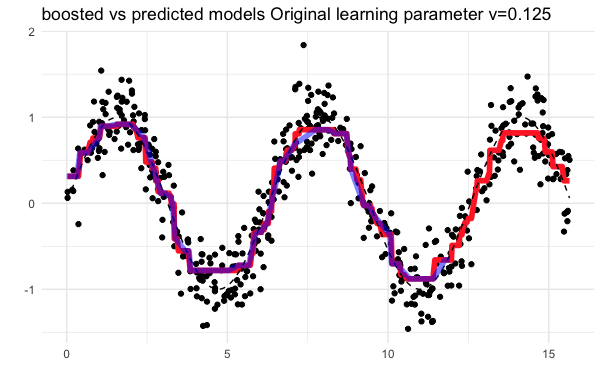
\includegraphics[width=16cm,height=10cm]{prediction_v_0.125.png}\\

As we observed, when the learning parameter is small, the overall model seems to be under-fitted, and the model progress slower by each learner than a relatively large learning parameter(v=0.125) \\

\item Q2 \\
\textbf{Part A} \\
The idea is to to check validation data RMSE during training stage, if we see the change in validation RMSE is small(the threshold is adjustable), we can early stop the training process. \\
Please refer to \textbf{tree-boosting-with-early-stop.R} script for the implementation. \\
\textbf{Part B} \\
If we set the validation RMSE change to be 0.005, the training stops with 30 trees in my case.\\ 
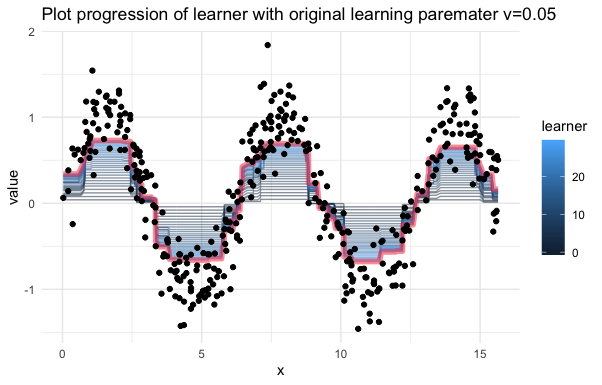
\includegraphics[width=16cm,height=10cm]{learner_v_0.05_warly_stop.png}\\

\textbf{Part C} \\
Test Data RMSE is .3549077 in my training.  \\

\item Q3 \\
Please refer to \textbf{tree-boosting-with-grid-search.R} for implementation. The best set of parameter is when minsplit=5, maxdepth=5 and cp=0.05, in such case, RMSE is 0.312280434490507 \\
\end{enumerate}
\item \textbf{Part2: Multiple-Dimension Case}
\begin{enumerate}
\item Q1 \\
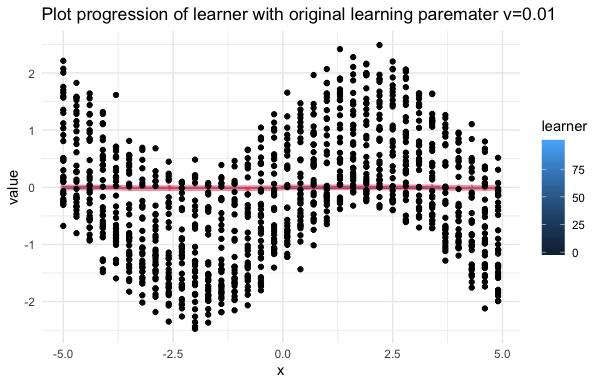
\includegraphics[width=16cm, height=10cm]{Multi_learner_v_0.01.png}\\
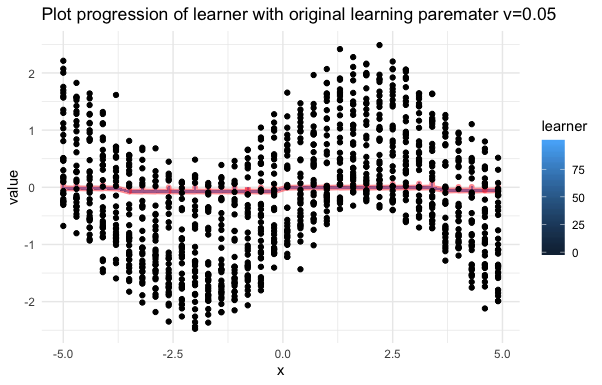
\includegraphics[width=16cm, height=10cm]{Multi_learner_v_0.05.png}\\
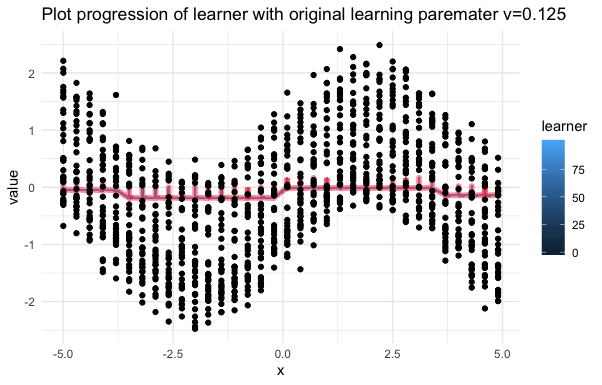
\includegraphics[width=16cm, height=10cm]{Multi_learner_v_0.125.png}\\
As we observed, the model seems to be under-fitted with current model.

\item Q2 \\
\textbf{Part A} \\
Please refer to \textbf{tree-boosting-multiple-dimension-early-stop.R} script for the implementation. \\
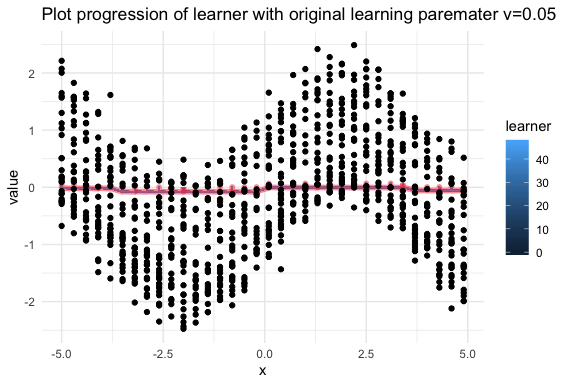
\includegraphics[width=16cm, height=10cm]{multiple_v_0.05.png}\\

\textbf{Part B} \\
48 trees are included. \\

\textbf{Part C} \\
RMSE for test dataset is 0.09576191. \\

\item Q3 \\
Please refer to \textbf{tree-boosting-multiple-dimension-grid-search.R} script for the implementation. \\

Please refer to \textbf{tree-boosting-with-grid-search.R} for implementation. The best set of parameter is when minsplit=2, maxdepth=5 and cp=0.01, in such case, RMSE is 0.101362044548129\\

\end{enumerate}
\end{enumerate}


\section{Question 2 (TSNE)}
\textbf{Part 1} \\
(a) Yes, it matters. It indicates that the two points are close in their original dimension space. \\
(b) It is an estimation of the amount of close neighbors each point has and can be user to balance attention between local and global aspects of your data. \\
(c) If the number of steps small, t-SNE plot may have  strange “pinched” shapes because it stops early and ends before convergence state. Optimal number of steps are dependent on data sample you have. \\
(d) read topological information off t-SNE plot typically requires views at multiple perplexities (multiple plots). One of the simplest topological properties is containment. t-SNE with low perplexity value greatly exaggerates the size of the smaller group of points. Another is trefoil knot, low perplexity values failed to show global connectivity.\\ 
\textbf{Part 2} \\
(a)\\
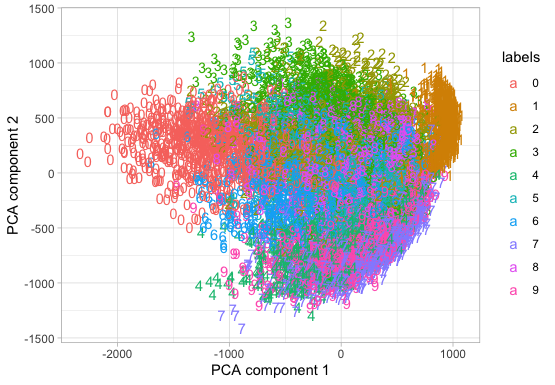
\includegraphics[width=16cm, height=10cm]{PCAPlot.png}\\
(b)\\ 
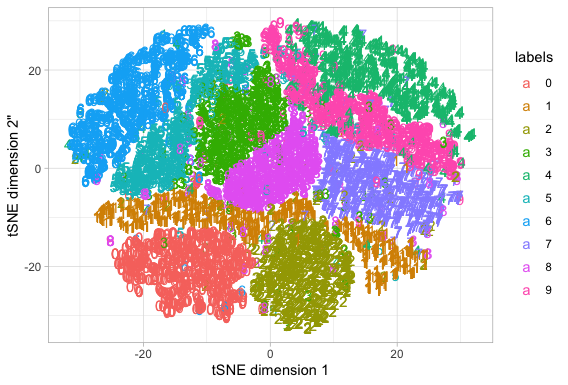
\includegraphics[width=16cm, height=10cm]{tSNE_5.png}\\
(c) \\ 
The following charts are shown when perlexity is 5, 20,60,100,125,160. \\
As we can see, the larger the perlexity, the more diverse each group is apart from each other. \\
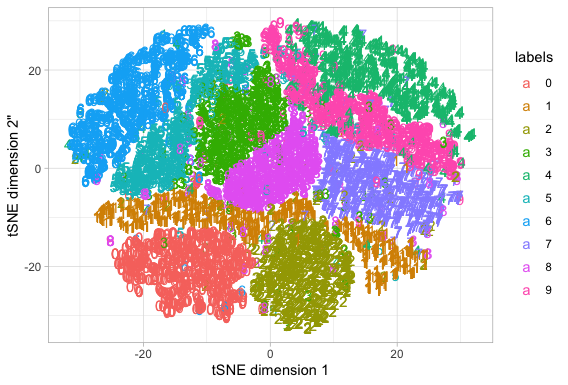
\includegraphics[width=16cm, height=10cm]{tSNE_5.png}\\
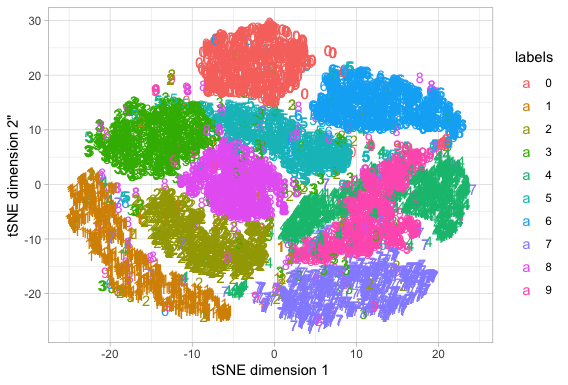
\includegraphics[width=16cm, height=10cm]{tSNE-20.png}\\
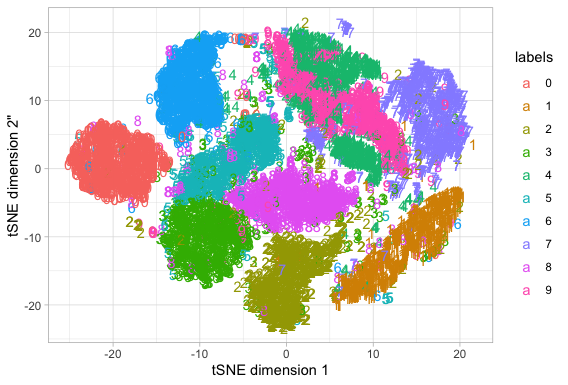
\includegraphics[width=16cm, height=10cm]{tSNE-60.png}\\
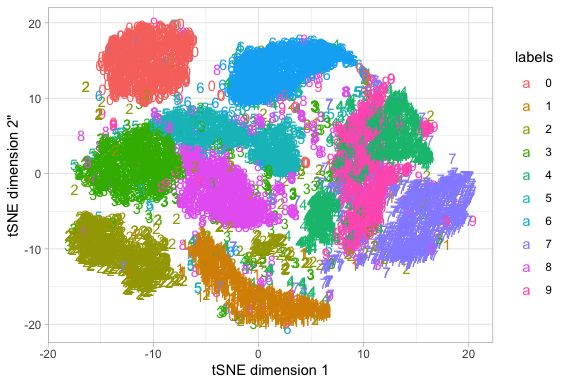
\includegraphics[width=16cm, height=10cm]{tSNE-100.png}\\
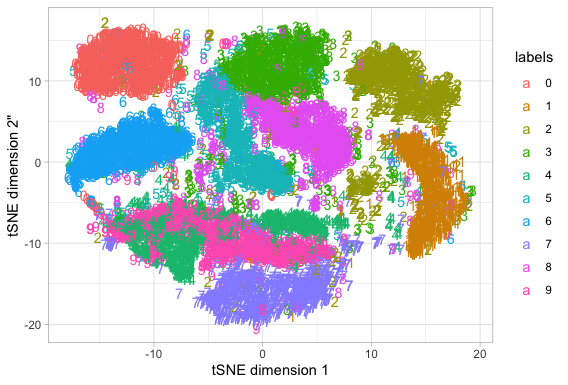
\includegraphics[width=16cm, height=10cm]{tSNE-125.png}\\
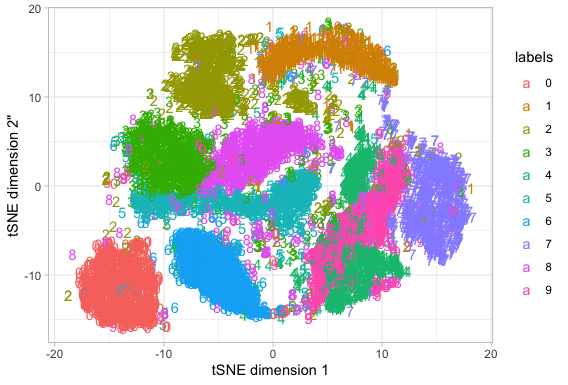
\includegraphics[width=16cm, height=10cm]{tSNE-160.png}\\
(d) \\ 
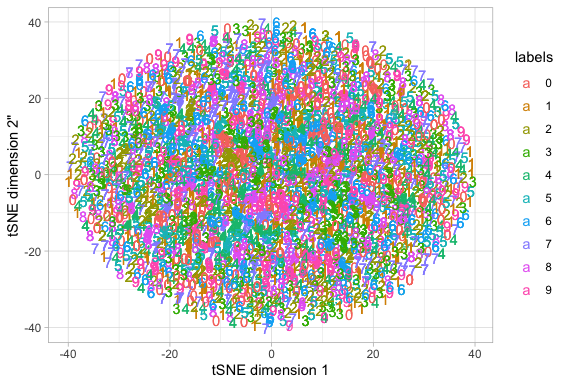
\includegraphics[width=16cm, height=10cm]{tSNE-1.png}\\
We can see that all the groups are mixed together, this means that we the perlexity is too small for the tSNE to converge. 
(e) \\
There will be clear decision boundaries between each group, they are totally seperable. \\
(f) \\
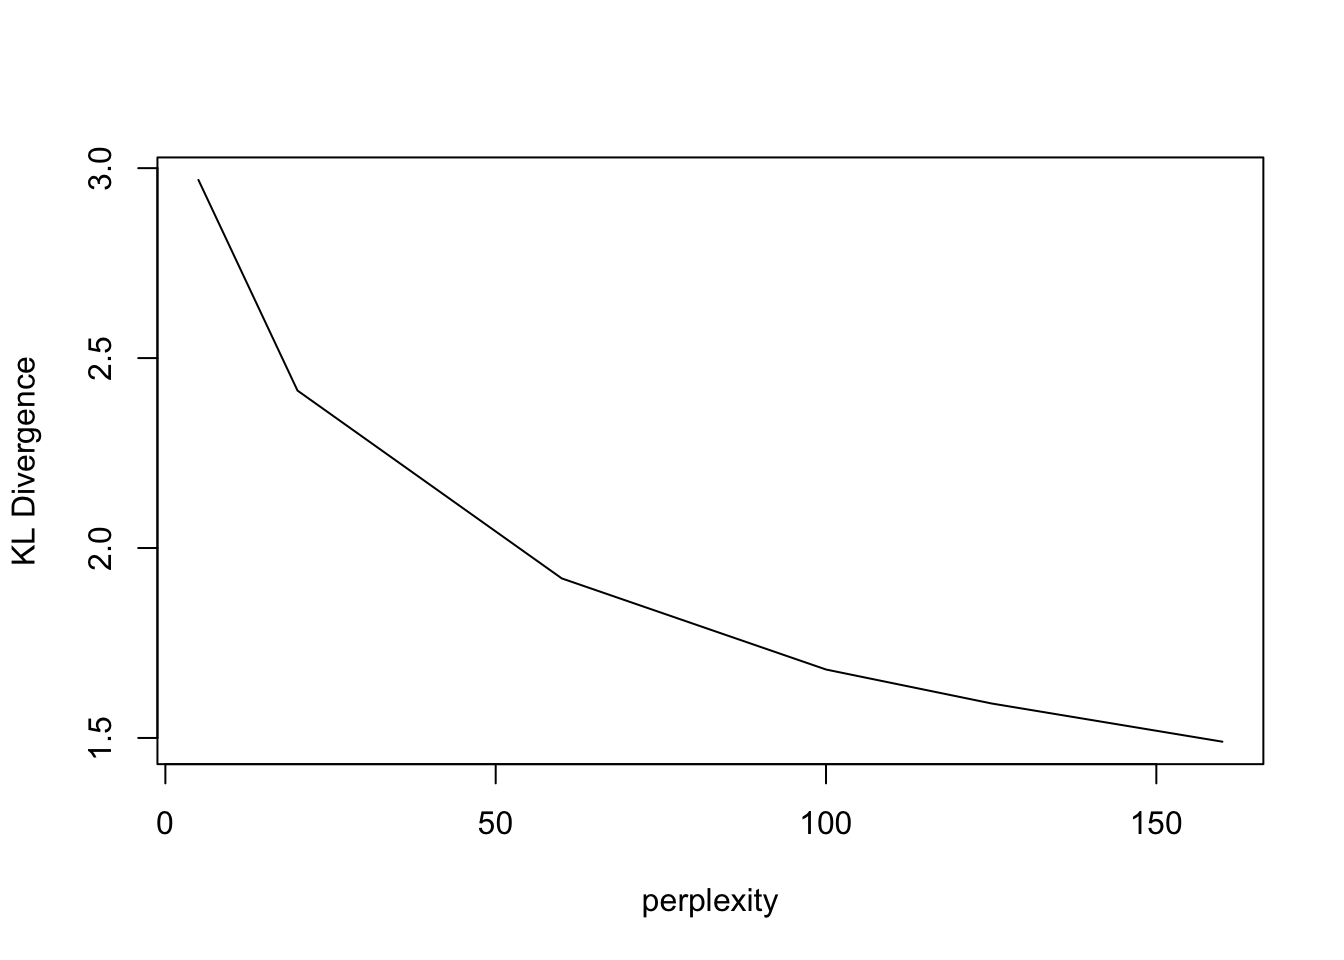
\includegraphics[width=16cm, height=10cm]{KLD-iteration.png}\\
The optimal perplexity is 160. \\
(g) \\
LARGER learning rate will lead to more dispersed clustering result.
Following are charts when eta=10, 100 and 200
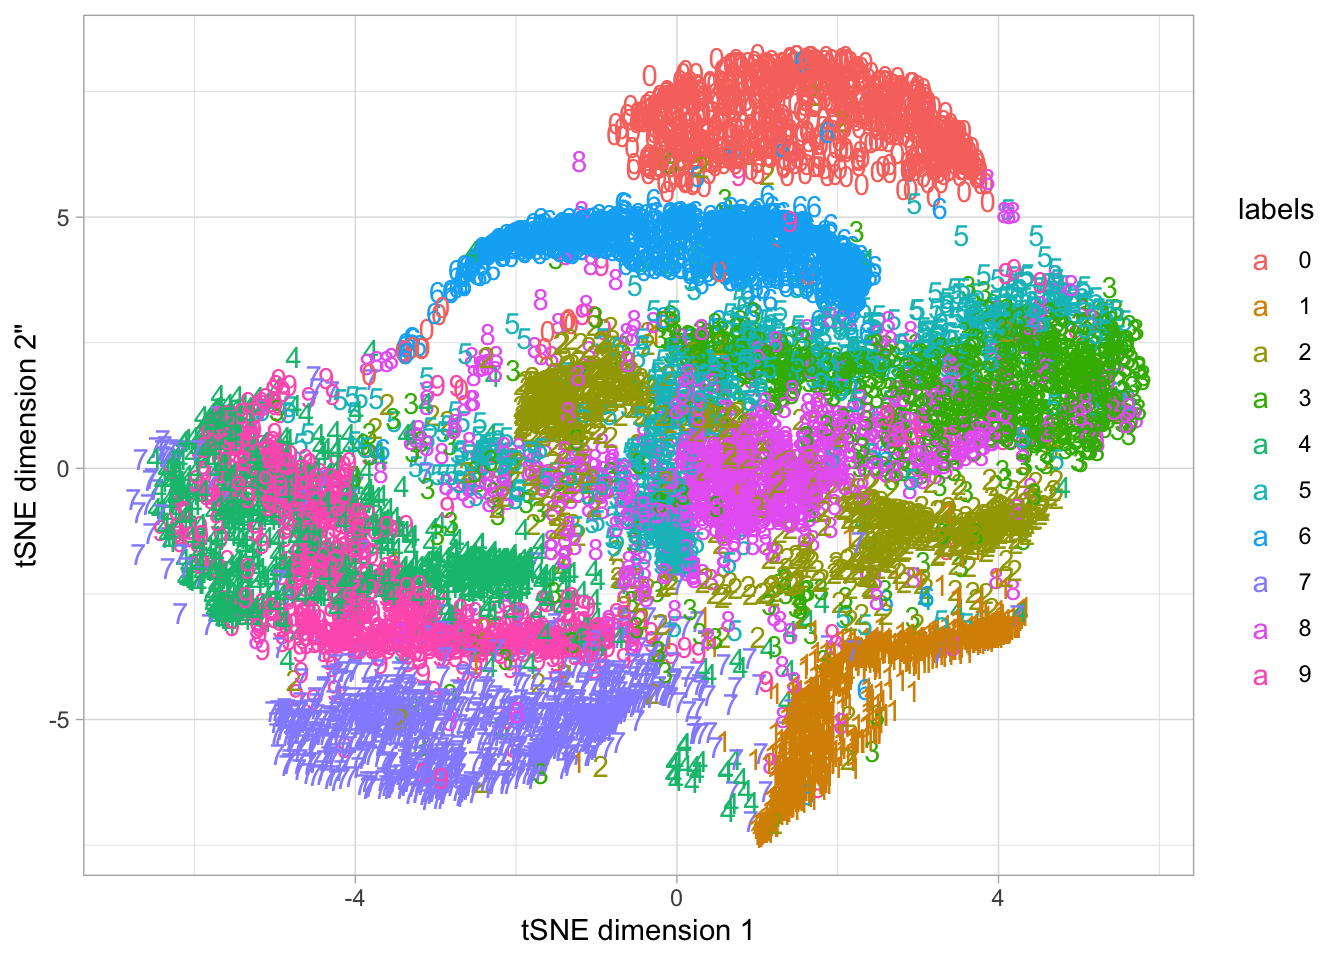
\includegraphics[width=16cm, height=10cm]{tsne-eta-10.png}\\
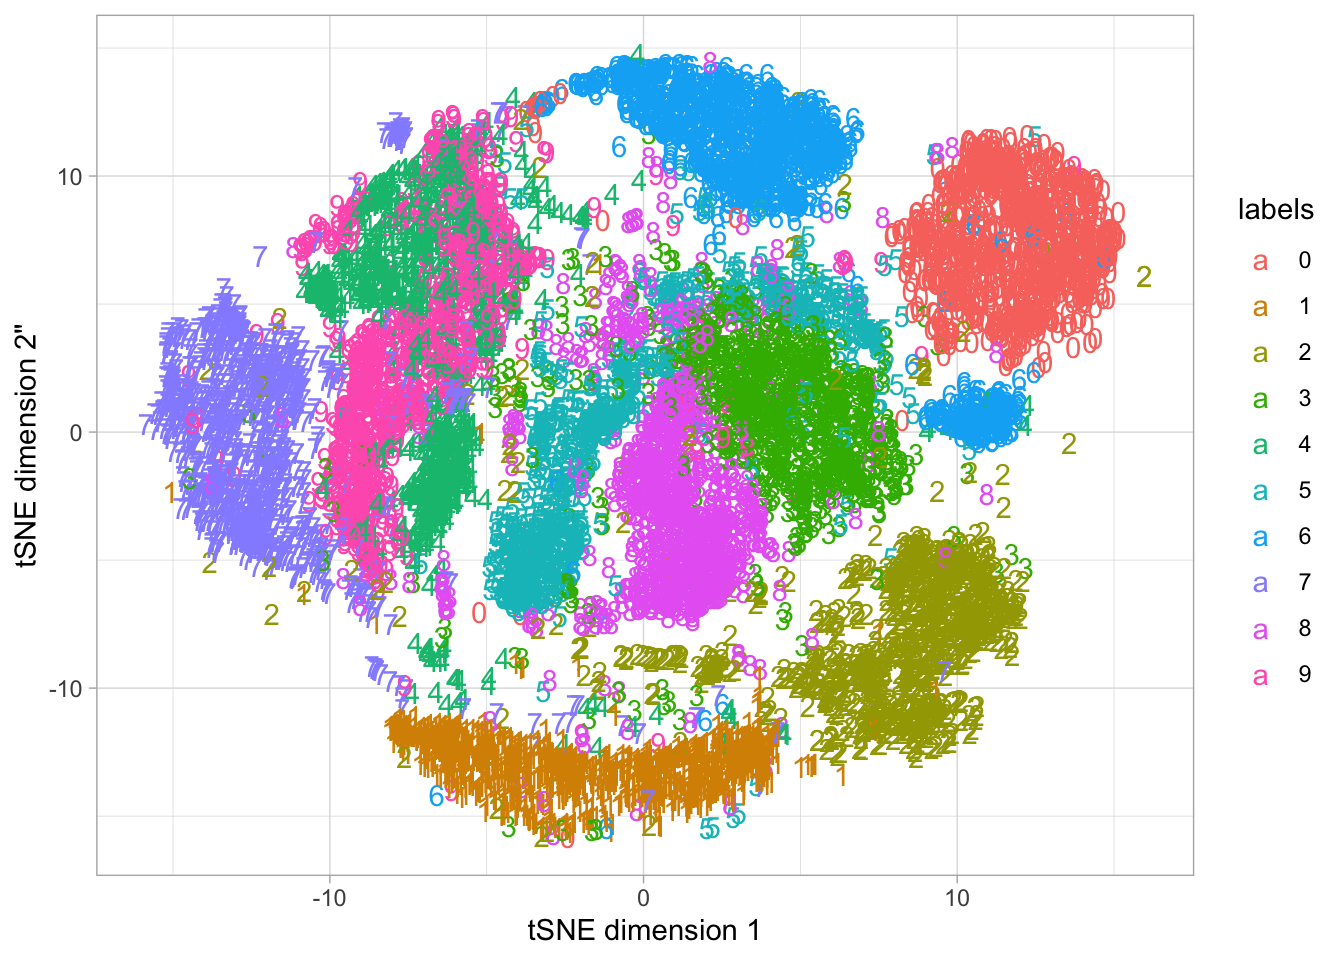
\includegraphics[width=16cm, height=10cm]{tsne-eta100.png}\\
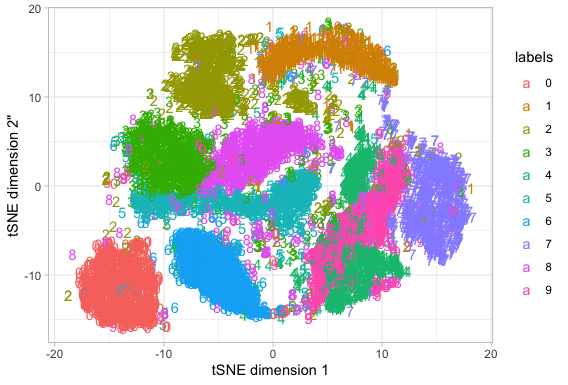
\includegraphics[width=16cm, height=10cm]{tSNE-160.png}\\

\section{Question 3 (Word2Vec) Emeddings} 
(1) \\
stop words removal, stemming or lemmatization and text normalization 

(2) \\
i chose BEAN, TOMATO and ONION as my ingredients. \\
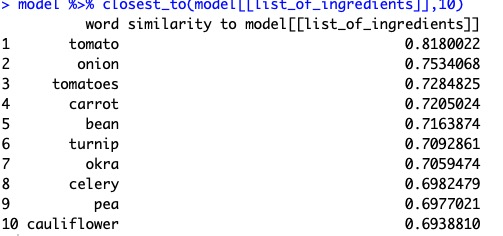
\includegraphics[width=16cm, height=10cm]{3.1.jpg}\\
tomato, onion, tomatoes, carrot, bean are the top 5 similar ingredient. \\
(3) \\
t-SNE to see the relationships between set of words related with the three ingredients above. \\
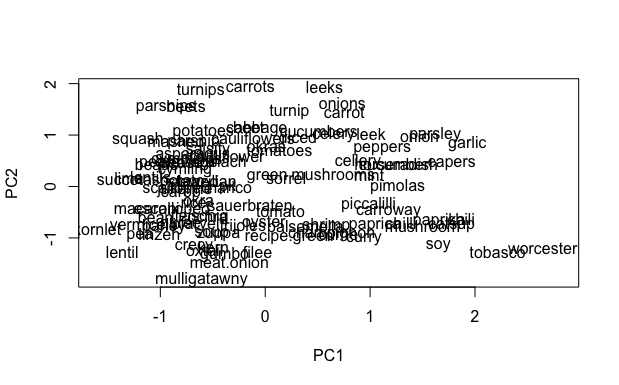
\includegraphics[width=16cm, height=10cm]{tSNE-3.3.png}\\
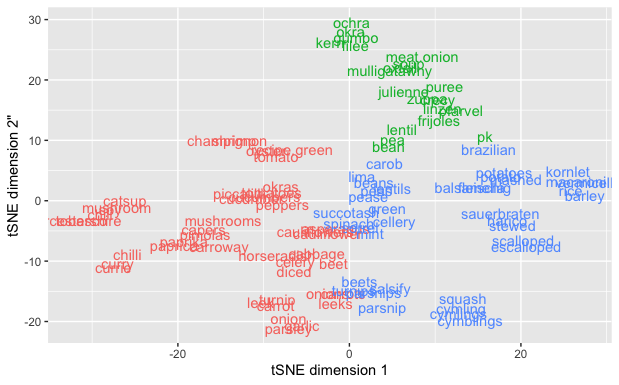
\includegraphics[width=16cm, height=10cm]{tSNE-3.2.2.png}\\

(4) \\
i use three tastes including hot, spicy and sour. \\
the results are reasonable in some way, however, the three cluster is not really as dispersed as previously. 
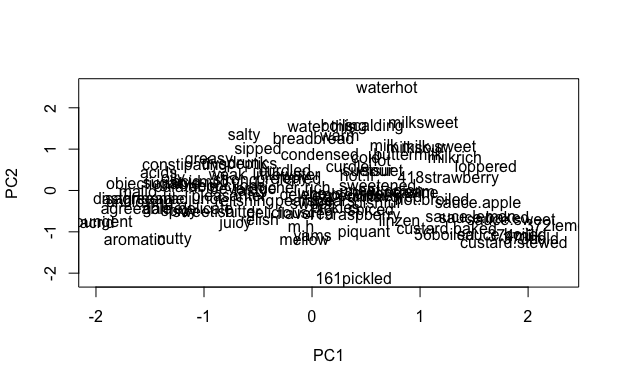
\includegraphics[width=16cm, height=10cm]{tsne-3.4.1.png}\\
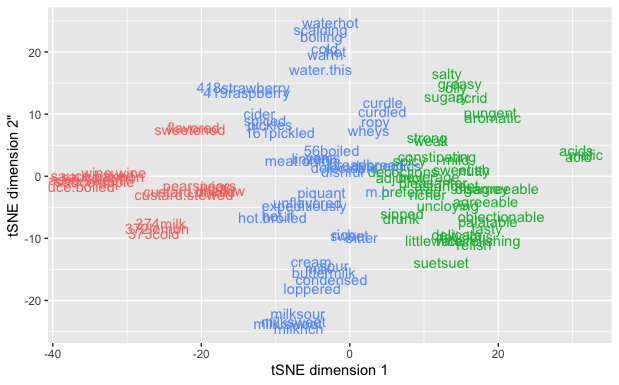
\includegraphics[width=16cm, height=10cm]{tune-3.4.2.png}\\

(5) \\
top_evaluative_words = model %>% 
  closest_to(~ "honey"+"toast",n=30) \\
goodness = model %>% 
  closest_to(~ "honey"-"toast",n=Inf) \\
taste = model %>% 
  closest_to(~ "egg" + "bread", n=Inf)\\
top_evaluative_words %>%
  inner_join(goodness) %>%
  inner_join(taste) %>%
  ggplot() + 
  geom_text(aes(x=`similarity to "honey" - "toast"`,
                y=`similarity to "egg" + "bread"`,
                label=word))\\
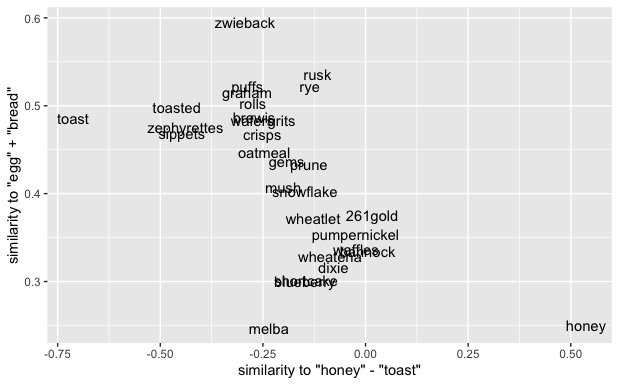
\includegraphics[width=16cm, height=10cm]{3.5.png}\\

(6) \\
we can see some interesting results like 'toast', 'oatmeal', as they are all common food for breakfast. \\
But its hard to imagine what is the relationship between '261 gold' with above words. \\

(7) \\
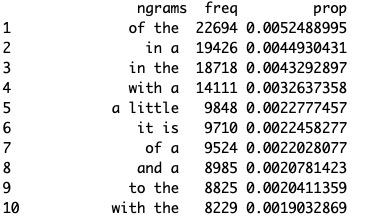
\includegraphics[width=16cm, height=10cm]{bigram.jpg}\\

\section{Question4 Gaussian Processes (Fitting a GP)} 
\textbf{Refer to Question4.R for implementation. } \\
\textbf{Part 1} \\
2. 
theta= 0.001 Negative Log Likelihood is 1872.595 \\
theta= 0.01 Negative Log Likelihood is 5976.789 \\
theta= 0.05 Negative Log Likelihood is 12251 \\
theta= 0.1 Negative Log Likelihood is 21813.76 \\
theta= 0.125 Negative Log Likelihood is 27880.98 \\
It is optimal when theta is 0.001. \\

3. \\
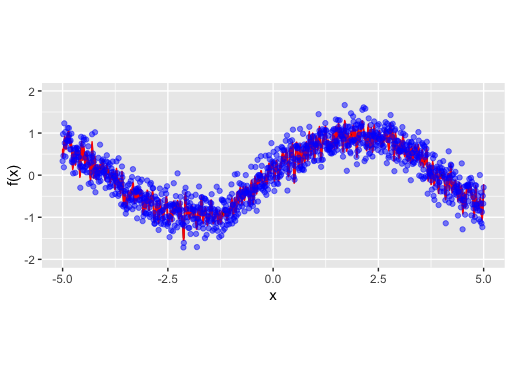
\includegraphics[width=16cm, height=10cm]{4.3.png}\\
\textbf{Part 2} \\

\section{Question5 Building Neural Networks} 
\textbf{Part 1: For a ReLu network} \\
\textbf{    Part 1.A: Losses} \\

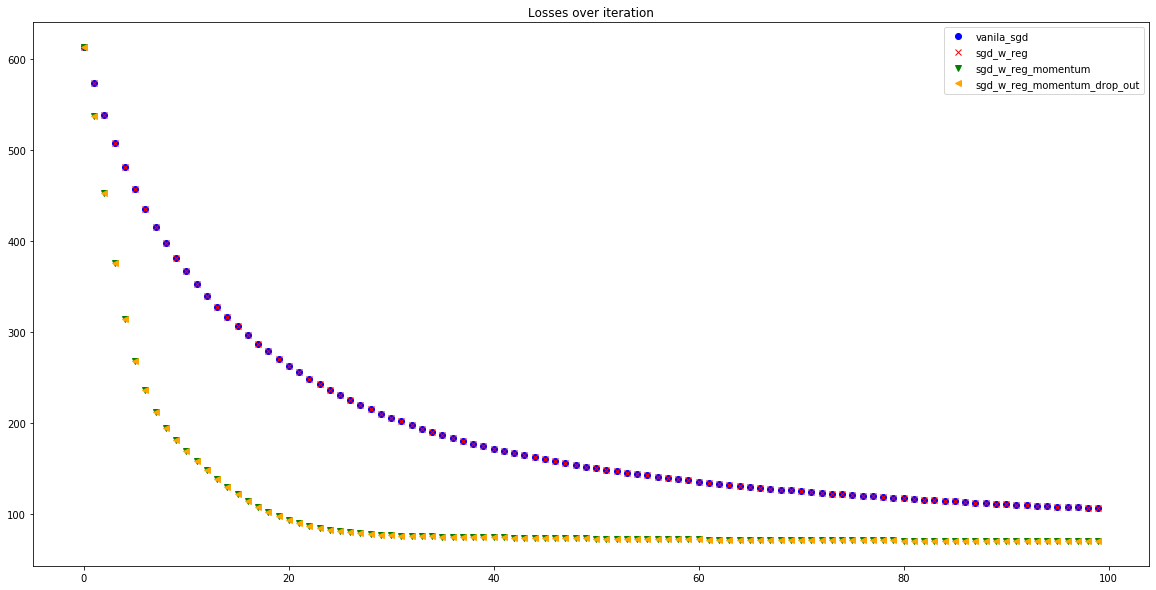
\includegraphics[width=16cm, height=10cm]{One_layer_losses_comparsion.png}\\
(a) As we observe above, vanilla-sgd and sgd-w-reg have relative similar performance, while sgd-w-momentum and sgd-w-reg-momentum-drop-out have similar performance and they are both better than the previous two methods.  And after 100 iterations, sgd-w-momentum and sgd-w-reg-momentum-drop-out achieved same loss.\\
(b) we can clearly see that momentum methods works better because Momentum helps accelerate gradients in the right direction during training process, thus with same number of iteration, we can see loss drops faster in momentum methods. \\
However, we can see both regularization and dropout does not affect the performance so much, this suggest that the model may be still under-fitted under 100 iterations. \\

\textbf{    Part 1.B: Losses when number of hidden node is 5} \\
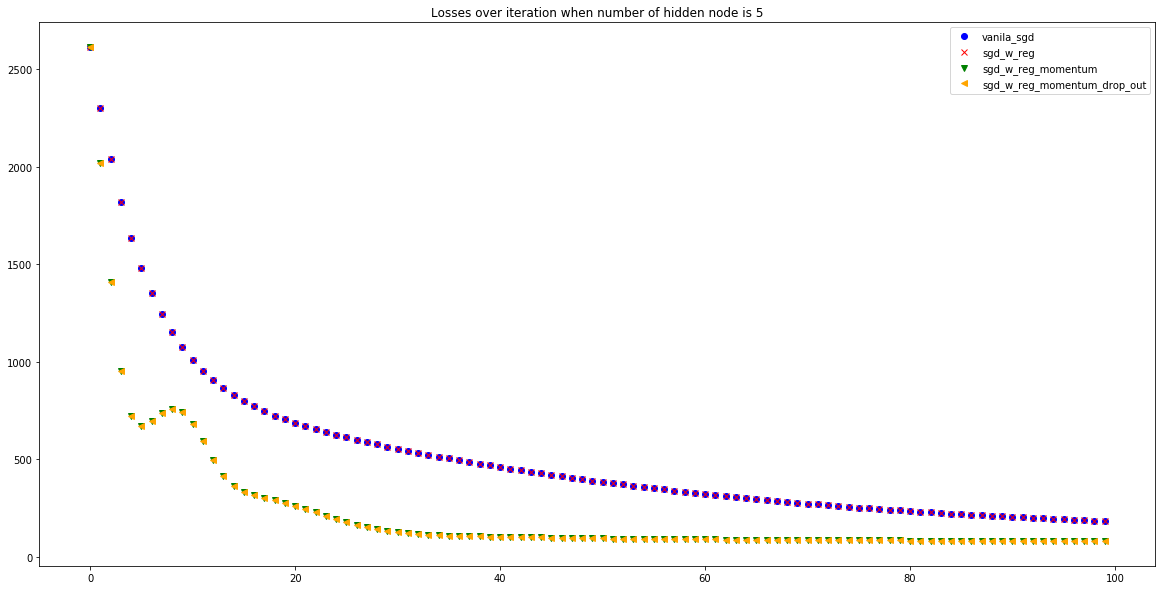
\includegraphics[width=16cm, height=10cm]{One_layer_losses_comparsion_5.png}\\
(a) And after 100 iterations, sgd-w-momentum and sgd-w-reg-momentum-drop-out achieved same loss. They are both better than the first two methods. \\
(b) The performance is not better than when number of hidden node is 3. This may suggests that the model starts to over-fit when number of hidden node is 5. \\
\textbf{Part 1.C: Run-Time comparison} \\

\begin{table}[htb]
\centering
\begin{tabular} { |s|p{2cm}|p{2cm}|  }
\textbf{Model} & \textbf{Time} \\ 
vanilla-sgd & 1.2593 \\
sgd-w-reg & 1.2183 \\
sgd-w-momentum  &  1.2227 \\ 
sgd-w-reg-momentum-drop-out & 1.2224
\end{tabular}
\end{table}\\

\textbf{Part 2: For a Sigmoid network} \\
\textbf{Part 2.A: Losses} \\
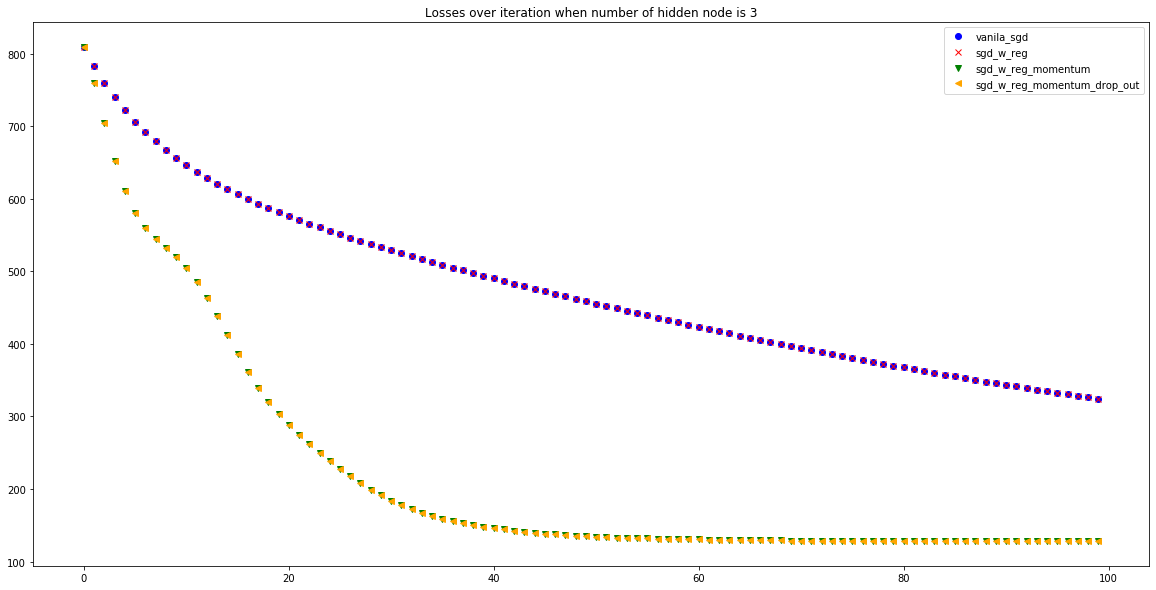
\includegraphics[width=16cm, height=10cm]{Sigmoid_3.png}\\

As we observe above, vanilla-sgd and sgd-w-reg have relative similar performance, while sgd-w-momentum and sgd-w-reg-momentum-drop-out have similar performance and they are both better than the previous two methods.  And after 100 iterations, sgd-w-momentum and sgd-w-reg-momentum-drop-out achieved same loss. \\

However, we can see both regularization and dropout does not affect the performance so much, this suggest that the model may be still under-fitted under 100 iterations. \\

\textbf{Part 2.B: Losses when number of hidden node is 5} \\
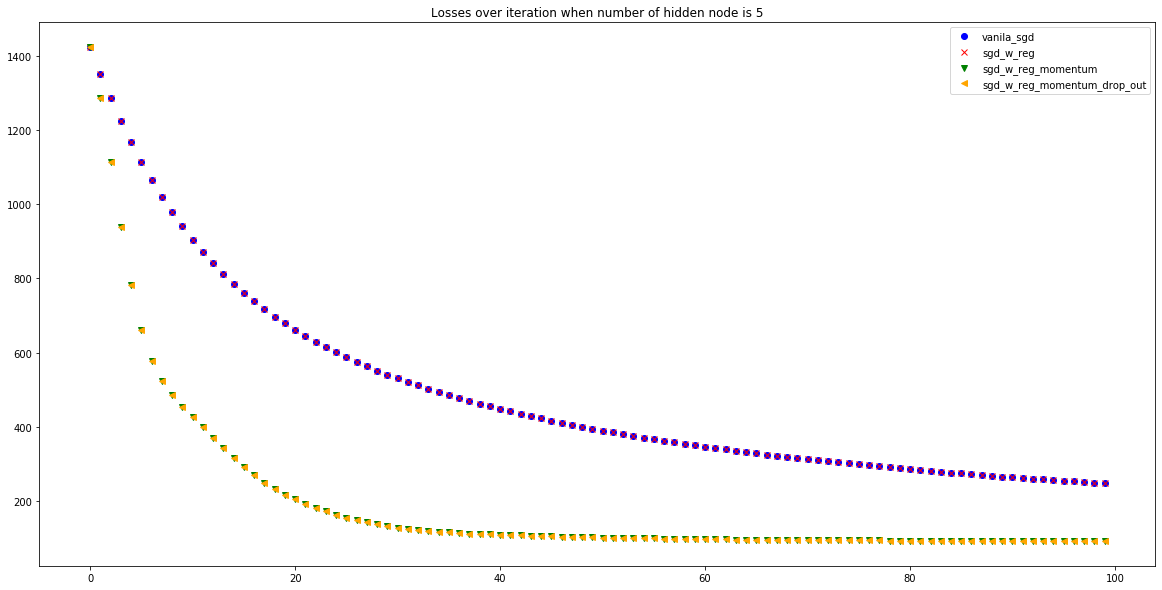
\includegraphics[width=16cm, height=10cm]{Sigmoid_5.png}\\
And after 100 iterations, sgd-w-momentum and sgd-w-reg-momentum-drop-out achieved same loss. They are both better than the first two methods. \\
This is better than when number of hidden node is 3, this means we need more complex models to learn better from the data. \\

\textbf{Part 2.C: Run-Time comparison} \\
\begin{table}[htb]
\centering
\begin{tabular} { |s|p{2cm}|p{2cm}|  }
\textbf{Model} & \textbf{Time} \\ 
vanilla-sgd & 1.2548 \\
sgd-w-reg & 1.2751 \\
sgd-w-momentum  &  1.2317 \\ 
sgd-w-reg-momentum-drop-out & 1.2653
\end{tabular}
\end{table}\\

\textbf{Part 2.D: Compare the performance of a ReLu network to a sigmoid network} \\
(1) 
\begin{table}[htb]
\centering
\begin{tabular} { |s|p{2cm}|p{2cm}|  }
\textbf{Model} & \textbf{3-node-Relu Loss} & \textbf{3-node-Sigmoid Loss} \\ 
vanilla-sgd & 106.058 & 324.282 \\
sgd-w-reg & 106.069 & 324.309 \\
sgd-w-momentum  &  69.996 & 128.640 \\ 
sgd-w-reg-momentum-drop-out & 69.996 & 128.640
\end{tabular}
\end{table}\\
Relu is generally better. \\

(2) 
\begin{table}[htb]
\centering
\begin{tabular} { |s|p{2cm}|p{2cm}|  }
\textbf{Model} & \textbf{5-node-Relu Loss} & \textbf{5-node-Sigmoid Loss} \\ 
vanilla-sgd & 182.366 & 247.184 \\
sgd-w-reg & 182.380 & 247.210 \\
sgd-w-momentum  &  79.418 & 91.377 \\ 
sgd-w-reg-momentum-drop-out & 79.418 & 91.377
\end{tabular}
\end{table}\\
Relu is generally better.  \\
(3) run time comparison on default parameter

\begin{table}[htb]
\centering
\begin{tabular} { |s|p{2cm}|p{2cm}|  }
\textbf{Model} & \textbf{3-node-Relu runtime} & \textbf{3-node-Sigmoid runtime} \\ 
vanilla-sgd & 1.2593 & 1.2548 \\
sgd-w-reg & 1.2183 & 1.2751 \\
sgd-w-momentum  &  1.2227 & 1.2317 \\ 
sgd-w-reg-momentum-drop-out & 1.2224 & 1.2653
\end{tabular}
\end{table}\\
run-time is comparable. \\
\section{Question 6 (Activation Functions)}
For the code simulation, refer to the Activation Function Study Jupyter Notebook.\\
\textbf{please be noted that those chart are generated from random data, and i picked up some of the most representative charts}

\textbf{part1} \\
\textbf{part1.a} \\
For one layer with one node, we have $y=V*Activation(wx+b)+v_b$: it has following possible shapes for Relu and Sigmoid. \\
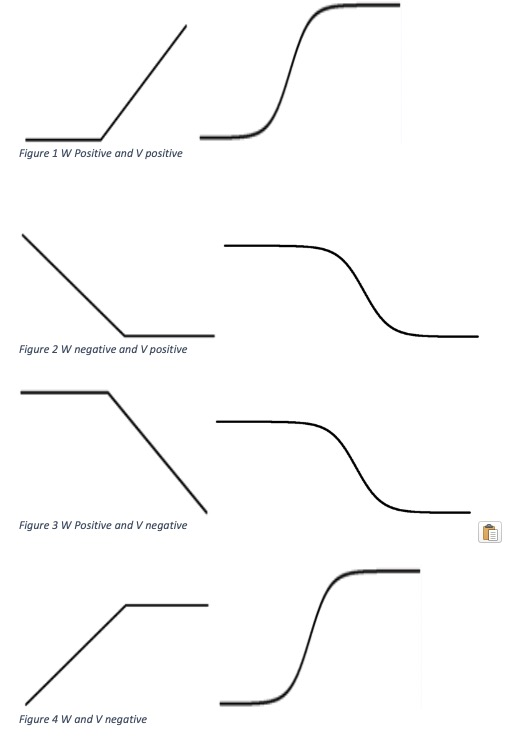
\includegraphics[width=16cm, height=16cm]{Onelayer_one_Node.jpg}\\
\textbf{part1.b} \\
For one layer with two node, we have $y=V_1*Activation(w_1x+b_1)+V_2*activation(w_2x+b_2)+v_b$: it has following possible shapes. \\
For ReLu: \\
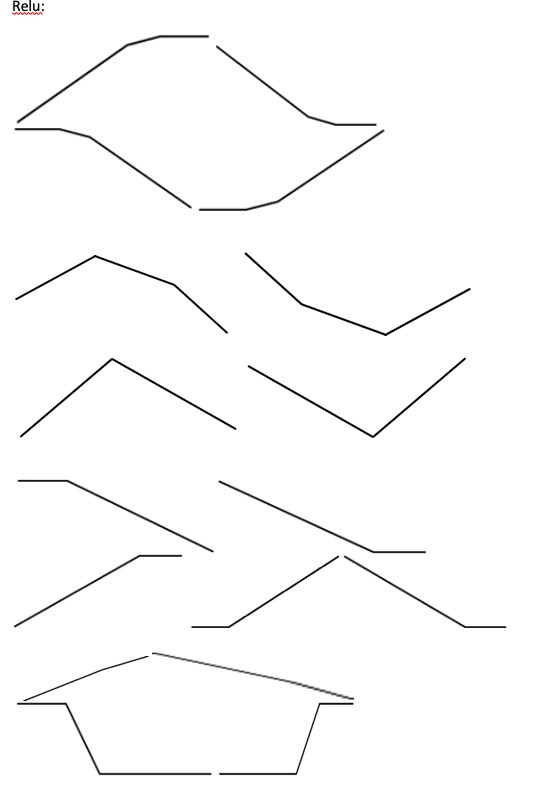
\includegraphics[width=16cm, height=16cm]{One_layer_Two_nodes.jpg} \\
For Sigmoid: 
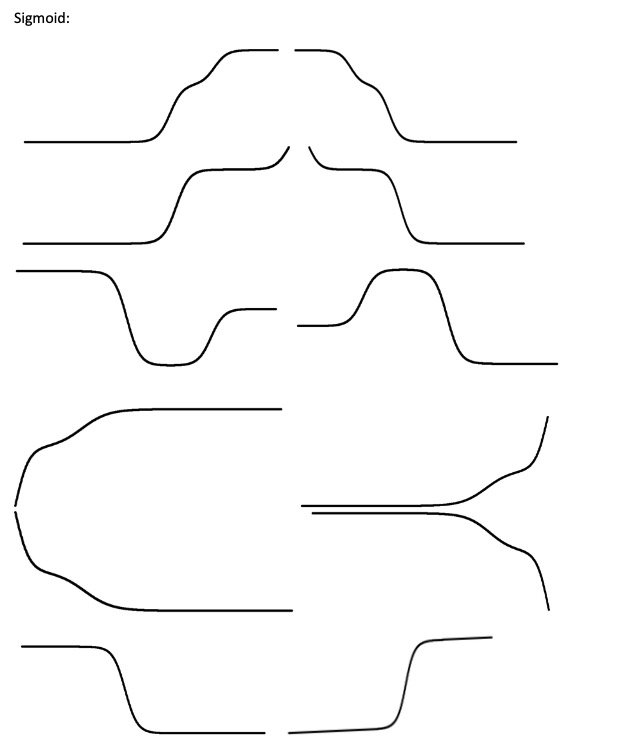
\includegraphics[width=16cm, height=16cm]{One_layer_two_node_sigmoid.jpg} \\
\textbf{part2} \\
\textbf{part2.a} \\
for two layers with one node, we have $y=v*Activation(w_2*activation(w_1*x+b_1)+b_2)+b$

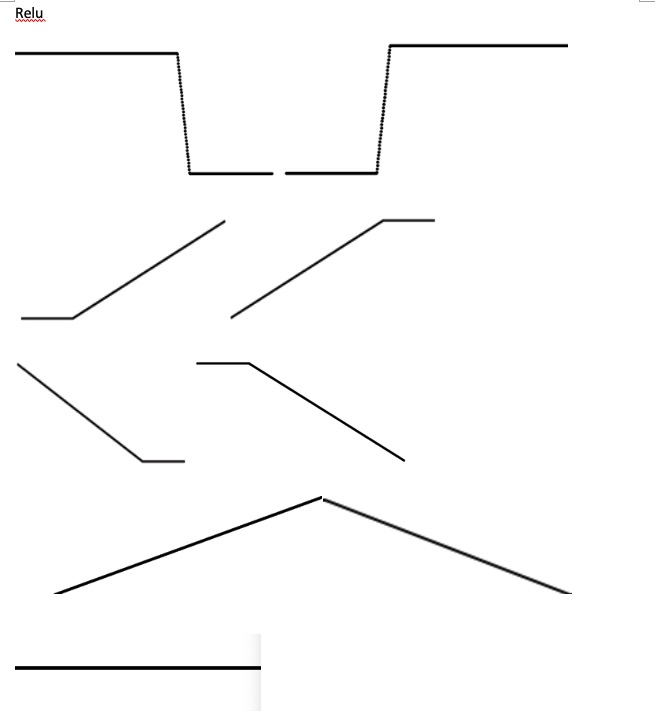
\includegraphics[width=16cm, height=16cm]{2_1_relu.jpg} \\
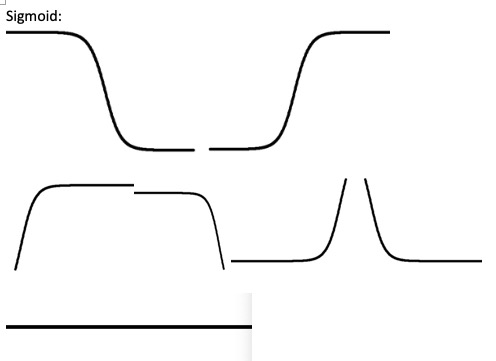
\includegraphics[width=16cm, height=16cm]{2_1_sigm.jpg} \\
\textbf{part2.b} \\
For this case, we will have $$
y=v1*acti(w11*acti(w1*x1+b1)+ \\ 
w21*acti(w2*x2+b2)+b21)+v2*acti(w12*acti(w1*x1+b1) \\
+ w22*acti(w2*x2+b2)+b22)+v_b
$$, 
we will have 8 weights terms and 5 bias term, there are a lot of possibilities. I have listed some of some for both Relu and Sigmoid.  \\
Generally, it could simulate a lot of functions with few spikes/valleys. It is hard to list down all possibilities. \\ 
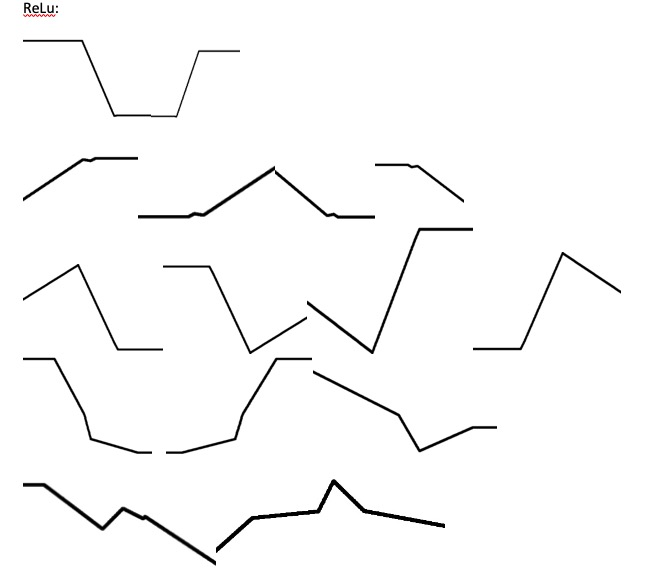
\includegraphics[width=16cm, height=16cm]{Relu_22.jpg} \\
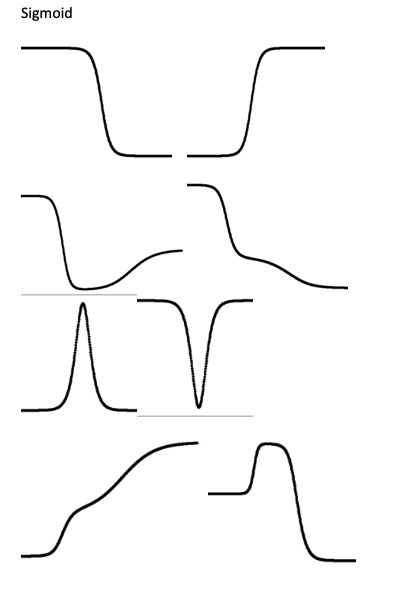
\includegraphics[width=16cm, height=16cm]{sigmoid_22.jpg} \\
\end{document}
